\documentclass{article}
\usepackage{graphicx}
\usepackage{listings}
\usepackage{tikz}
\usetikzlibrary{positioning,fit,calc}
\tikzset{block/.style={draw,thick,text width=2cm,minimum height=1cm,align=center},
         line/.style={-latex}
}
\begin{document}

\title{CM30171}
\author{Rob Willison}

\maketitle
\tableofcontents

\section{Overview}
This report is an explanation of the design decisions undertaken while writing
a --C compiler and interpreter. The project was written in C and involves three
different sections of code, an interpreter, TAC compiler and MIPS compiler.\\~\\

The interpreter for --C handles functions, closures, if - else statements and while loops.
It uses an environment comprised of frames to store variable values in different scopes. Each
variable can either be a integer or closure. The major design decisions in the interpreter
include the design 

The TAC Compiler performs a walk over the AST at each node a section of TAC is created.
The TAC is separated into blocks between each label and jump, this allows next use
information to be generated in order for easy TAC optimisation.\\~\\
For the MIPS the problem of delayed branching was ignored to simplify the compiler
and due to time constraints I didn't get round to adding the required nops into the
compiler.

\newpage
\section{Code Interpretation}

In order to interpret --C code the abstract syntax tree is walked, at each node
the left and right children are compiled and the nodes operation is applied to them.
In order to support both integer and closure return types all the functions which handle
node interpretation return a union structure which either contains the integer value or
a pointer to the closure. The interpreter supports variable assignment, closures, if-else and while
statements I will explain each now.

\subsection{Variable Assignment}
In order to store a value an environment structure was implemented this consists
of a list of frames, one for each scope in the program, and each frame contains a
list of bindings of token to union. The environment is added to each type a variable
assignment is made and new frames are added each time a new scope is entered, frames are
removed from the list when this scope is left.

\subsection{Closures \& Functions}
In order to store and call closures there is a closure structure this holds a pointer
to the environment frame the closure was defined in and also a pointer to the start node
of the AST that defines the function. Then when a closure is applied the variable is pulled
out of the environment and the AST interpreted with the environment it was defined with.\\~\\
The interpretation of the functions AST continues until a return node is found, at
this point the hasReturned field is set. When the has returned field is set
no other lines of code in the current function are executed and the function returns this
value.

\subsection{Control Structure}
There are two types of control structure in --C the if-else and while loop.
In order to interpret an if - else statement the condition is interpreted and depending on
if the value is non-zero or not either the right or left child.\\
For the while loop firstly the conditional is returned then the body, this is repeated
while the conditional is non-zero.



\section{Intermediate Code Generation}

\subsection{TAC Design}

The three address code used in the compiler was designed to be abstract enough as
too keep any machine dependent decisions out of the TAC stage. Many of the instructions
are obvious such as store and mathematic operations, examples below, and they won't be explained in
great detail.

\begin{lstlisting}
r2 := 1
r3 := r1 / r2
\end{lstlisting}

One thing to note about the store instruction is that in the event that the store
operand is defined in the scope above the current scope like x is in the following example.

\begin{lstlisting}
int main()
{
  int x = 4;
  int test()
  {
    return x;
  }

  return test();
}
\end{lstlisting}

In that scenario the store command in the test function will have an extra piece
of information saying that its defined in the scope one level above, so the store command will
look like the following.

\begin{lstlisting}
DEFINED IN 1 r2 := x
\end{lstlisting}

This information is also included when a closure is called from a narrower scope,
the TAC would be as follows.

\begin{lstlisting}
CALL _1 FROM SCOPE 1
\end{lstlisting}

For Functions a label instruction denotes the start and a end label for the end.
After the start label the new activation frame instruction which tells
the compiler to allocate space for a new activation frame with a given number
of arguments, locals and tempories. Before the end there is a return instruction
which contains the register with the value to return. Below is an example function
in TAC.

\begin{lstlisting}
_1:
NEW FRAME 0 arg 0 loc 1 temp
DEFINED IN 1 r2 := x
RETURN r2
FUNCTION END
\end{lstlisting}

There is one type of control sequence in the language, the if else, the way this
is described in TAC is using a sequence of if instructions and labels denoting the
various bodies if the if and else parts. An example in --C and the corresponding TAC
are below.

\begin{lstlisting}
if (1 > 4) {
  return 4;
} else if (2 > 1) {
  return 3;
}
\end{lstlisting}

\begin{lstlisting}
r1 := 1
r2 := 4
r3 := 1 > 4
IF NOT r3 GOTO 1
r4 := 4
RETURN 4
GOTO 2
LABEL 1: r5 := 2
r6 := 1
r7 := 2 > 1
IF NOT r7 GOTO 3
r8 := 3
RETURN 3
LABEL 3: LABEL 2:
\end{lstlisting}

Finally there is one loop type in the language, the while loop, this is translated
into a goto, an if and a label at the top and bottom of the loop body. the while
condition is placed after the body. n example in --C and the corresponding TAC
are below.

\begin{lstlisting}
int x = 0;
while (x < 5)
{
  x = x + 1;
}
\end{lstlisting}

\begin{lstlisting}
r1 := 0
x := r1
GOTO 1
LABEL 2: r2 := x
r3 := 1
r4 := r2 + r3
x := r4
LABEL 1: r5 := x
r6 := 5
r7 := r5 < r6
IF r7 GOTO 2
\end{lstlisting}

\subsubsection{List of TAC instuctions}
\begin{lstlisting}
x := y                            Store the value of y in x
x := y + z                        Store the result of y + z in x
x := y - z                        Store the result of y - z in x
x := y * z                        Store the result of y * z in x
x := y / z                        Store the result of y / z in x
x := y < z                        Store the result of y < z in x
x := y > z                        Store the result of y > z in x
x := y >= z                       SStore the result of y <= z in x
x := y <= z                       Store the result of y >= z in x
LABEL x:                          Create a label with the name x
GOTO x                            jump to the label with name x
IF NOT x GOTO y                   If x has the value 0 jump to y
CREATE CLOSURE x                  define closure with the code label x
x:                                Also a label of value x
ALLOCATE PARAMS x                 Allocate a space for x parameters
SAVE PARAM x                      Save x in the next parameter space
NEW FRAME x arg y loc z temp      Allocate space for the activation frame
RETURN x                          Return the value in x
FUNCTION END                      A tag for the end of the function
\end{lstlisting}


\subsection{TAC Generation}

All the TAC complilation is done in the tac\_compliler.c file.
In order to generate the TAC from source code a tree walk is performed over the
parse tree at each node depending on the type a set of TAC instructions are created
and added to the current TAC block. If a new function is found a new TAC block is
created before that part of the tree is parsed, also if a goto or label TAC instruction
are created new blocks are created. When a leaf is reached a store instruction is
created for the value at the leaf.\\~\\

\subsubsection{Enviroment Structure}

In order to keep track of the location of any local variables in the code and enviroment
is created to store the association between token and register location. The enviroment
is made up of frames each frame corresponds to a scope in the program and has
a linked list of all locals in that scope. The frames also contain a linked list of
the functions defined, these are a pair of token and label assigned to the function.
For example the environment created while walking the following piece of code is shown below.

\begin{lstlisting}
int main()
{
  int x = 4;
  int test()
  {
    int y = 5;
    return x * y;
  }

  return test();
}
\end{lstlisting}

\begin{tikzpicture}
  \node[block] (a) {Frame 1};
  \node[block,right=of a] (b) {Frame 2};
  \node[block] (c) at [yshift=-2cm] {x - r1};
  \node[block] (d) at [yshift=-4cm] {test - \_0};
  \node[block, right=of a] (e) at [yshift=-2cm, xshift=1.2cm] {y - r2};
  \draw[line] (a)-- (b);
  \draw[line] (a)-- (c);
  \draw[line] (c)-- (d);
  \draw[line] (b)-- (e);
\end{tikzpicture}

As you can see the environment holds the association between the tokens of the variables
and functions with the TAC register location and the function label respectively.

\subsubsection{TAC Blocking}

The diffrent blocks of TAC code, between labels and jumps, are separated to allow
easier optimisation and MIPS translation. As the AST is walked if a instruction which
requires a jump (If, While, Function Call) is found a new block is created and set as the
current block after the jump. Similarly if a label is created a new block is created
and the label is assigned to that new block.\\~\\
in order to compile the code in the same order as the TAC each block has a link to
the block which was created from the code directly after it. A Simple example is
given below.\\~\\

\begin{center}
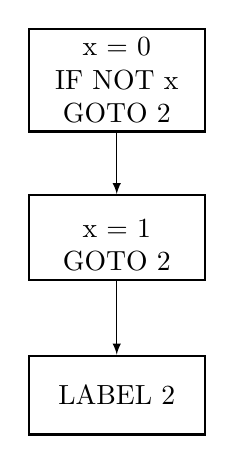
\begin{tikzpicture}
  \node[block] (a) {x = 0\\ IF NOT x GOTO 2};
  \node[block] [yshift=-2cm] (b) {\\ x = 1\\ GOTO 2};
  \node[block] [yshift=-4cm] (c) {LABEL 2};
  \draw[line] (a)-- (b);
  \draw[line] (b)-- (c);
\end{tikzpicture}
\end{center}

This was done so that the MIPS compilation step can easily follow the sequence of
TAC instructions. //TODO write about linking blocks if and when done

\subsubsection{Inner functions}

In order to implement inner functions, functions defined inside another, in TAC
the code for the function must be flattened so that there are no functions in functions
in the TAC. To do this when a function definition is reached inside another the current
TAC block is stored and another is created for the inner function, once the inner function's
AST has finished being walked the previous block is restored as the current block and
the AST tree walk continues. This gives the result of placing any inner functions after
the function it was defined in.

\subsection{Next Use Info}

As the TAC instructions are broken down into blocks next use informationn can be
worked out to allow optimisation. The next use info for a block is calculated by
using a recursive function which looks at each instruction in term from bottom
to top. A list of NEXT\_USE\_INFO structures is used, one structure for each variable
used in the block. Each NEXT\_USE\_INFO structure contains a list of the uses of that
variable and the associated liveness at that point. This is all done in the nextUseInfo.c file.

\subsection{TAC Optimisation}

After the TAC generation phase has been completed the sequence of blocks is handed
over to the optimisation phase. This is in the tac\_optimiser.c file. This applies
constant folding, copy propagation, dead code elimination, common sub expression
elimination and algebraic transformations algorithms to the TAC block repeatedly till
now change can be made. Each TAC block is processed from bottom to top for each
optimisation technique.

\subsubsection{Copy Propagation}

Copy propagation looks for a store instruction, once on is found it checks the
rest of the code below the store until it finds a write to the store destination.
For every read of the destination before replaced the use is replaced with the
stores operand. To demonstrate this copy propergation was applied to the same example
as above.

\begin{minipage}{0.3\textwidth}
\begin{lstlisting}

int x = 4;
int y = 6;

return x + y;

\end{lstlisting}
\end{minipage}%
\begin{minipage}{0.3\textwidth}
\begin{lstlisting}
r1 := 4
x := r1
r2 := 6
y := r2
r3 := x
r4 := y
r5 := r3 + r4
RETURN r5

\end{lstlisting}
\end{minipage}%
\begin{minipage}{0.3\textwidth}
\begin{lstlisting}
r1 := 4
x := 4
r2 := 6
y := 6
r3 := 4
r4 := 6
r5 := 4 + 6
RETURN r5
\end{lstlisting}
\end{minipage}%

\subsubsection{Constant Folding}

The constant folding function looks for arithmetic operations and replaces them
with the result where possible. This is done by looking for a operation where both
operands are tokens with type constant. Below is an example using both constant
folding and copy propergation.

\begin{minipage}{0.3\textwidth}
\begin{lstlisting}

int x = 4;
int y = 6;

return x + y;

\end{lstlisting}
\end{minipage}%
\begin{minipage}{0.3\textwidth}
\begin{lstlisting}
r1 := 4
x := 4
r2 := 6
y := 6
r3 := 4
r4 := 6
r5 := 4 + 6
RETURN r5

\end{lstlisting}
\end{minipage}%
\begin{minipage}{0.3\textwidth}
\begin{lstlisting}
r1 := 4
x := 4
r2 := 6
y := 6
r3 := 4
r4 := 6
r5 := 10
RETURN 10
\end{lstlisting}
\end{minipage}%

\subsubsection{Dead Code Elimination}

Dead code elimination works by analysing each instruction using and useing the
next use info removes them if not needed. Firstly this is only done for registers
user defined variables are live at the end of the block so an't removed. A instruction
is removed if the next use is not live, its another write, or there isn't another
next use. Using the same example as above and applying dead code elimination gives
the following.

\begin{minipage}{0.3\textwidth}
\begin{lstlisting}

int x = 4;
int y = 6;

return x + y;

\end{lstlisting}
\end{minipage}%
\begin{minipage}{0.3\textwidth}
\begin{lstlisting}
r1 := 4
x := 4
r2 := 6
y := 6
r3 := 4
r4 := 6
r5 := 10
RETURN 10

\end{lstlisting}
\end{minipage}%
\begin{minipage}{0.3\textwidth}
\begin{lstlisting}
RETURN 10
\end{lstlisting}
\end{minipage}%

The function which completed the dead code elimination step does not recalculate
the number of tempories in the code. So when the activation record is allocated
it will be for the original number of registers, which can waste a lot of memory.
This would be easy to recompute but I ran out of time.

\subsubsection{Common Sub Expression Elimination}
If two expression have the same operands and operation the later one can be replaced
with a store of the destination of the first. These are found by looking for pairs
of arithmatic operations, when one is found if the operation and operands are the
same the second is replaced with a store. An exaple is given below usign this method
in conjunction with copy propergation.

\begin{minipage}{0.3\textwidth}
\begin{lstlisting}

int c = 4 * 6;
int d = 4 * 6;

return c;

\end{lstlisting}
\end{minipage}%
\begin{minipage}{0.3\textwidth}
\begin{lstlisting}
r1 := 4
r2 := 6
r3 := r1 * r2
c := r3
r4 := 4
r5 := 6
r6 := r4 * r5
d := r6
r7 := c
RETURN r7
\end{lstlisting}
\end{minipage}%
\begin{minipage}{0.3\textwidth}
\begin{lstlisting}
r1 := 4
r2 := 6
r3 := 4 * 6
c := r3
r4 := 4
r5 := 6
r6 := r3
d := r3
r7 := r3
RETURN r3
\end{lstlisting}
\end{minipage}%

\subsubsection{Algebraic Transformations}

The final optimisation technique is to transform some algebraic expressions
which will always give 1 or 0 to those values. In order to do this the optimiser
looks for those specific expressions and simply replaces them with a store of either
1 or 0 depending on the expression. An example is given below using copy propagation
aswell.

\begin{minipage}{0.3\textwidth}
\begin{lstlisting}

int x = test();
int a = 0 + x;

return a;
\end{lstlisting}
\end{minipage}%
\begin{minipage}{0.3\textwidth}
\begin{lstlisting}
CALL _1
r2 := result
x := result
r3 := 0
r4 := result
r5 := 0 + result
a := r5
r6 := r5
RETURN r5
\end{lstlisting}
\end{minipage}%
\begin{minipage}{0.3\textwidth}
\begin{lstlisting}
CALL _1
r2 := result
x := result
r3 := 0
r4 := result
r5 := result
a := result
r6 := result
RETURN result
\end{lstlisting}
\end{minipage}%

\section{Machine Code Generation}

After the TAC is generated and optimised the code is translated to MIPS
assembler. This is done block by block in the order the TAC was generated.
Before the user code is compiled a global MIPS block is added which allocates memory
for global scope functions and sets up the environment used for variable lookup.\\
A decision was made to store all variables in memory and ignore the problem of register
assignment, this makes the compiler simpler however reduces its performance. The files
associated with this section of the compiler are compiler.c and MIPS.c.\\
In order for the users code to be run the main function has to be found as it
was renamed by the TAC to _0. A mips main function is added at the head of the mips
this contains a dynamic allocation of memory for the global scope functions, it then
fills these spaces with the functions. After this it calls the function _0, the users
main function.

\subsubsection{Functions}
When a function is compiled the first thing that happens is the number of locals,
temporaries and arguments are counted and a space big enough for all these is allocated.
This activation frame also contains space for the return address, previous frame
and enclosing frame. These are structured as shown in the diagram below.

//TODO draw diagram

One this is created and the first 3 spaces filled the arguments are all loaded
into the next spaces in the frame. Any arguments are loaded from the memory pointed
by \$a0. The function code is then compiled. The final
section of the code is to return to the calling code, any result is moved to \$v0
the previous frame is restored into the \$fp and the return address jumped to.\\
Below is a simple function example in mips with annotations.

\begin{minipage}{0.4\textwidth}
\begin{lstlisting}

int times(int n, int d)
{
  return n * d;
}

\end{lstlisting}
\end{minipage}%
\begin{minipage}{0.6\textwidth}
\begin{lstlisting}
function1:      (1)
move $t2 $a0    (2)
li $a0 40       (3)
li $v0 9        (4)
syscall         (6)
move $t0 $fp    (5)
move $fp $v0    (6)
sw $t0 0($fp)   (7)
sw $ra 4($fp)   (8)
sw $a1 8($fp)   (9)
lw $t1 0($t2)   (10)
sw $t1 12($fp)
lw $t1 4($t2)
sw $t1 16($fp)
lw $t1 12($fp)  (11)
lw $t2 16($fp)
mult $t1 $t2
mflo $t0
sw $t0 20($fp)
lw $v0 20($fp)  (12)
lw $t0 4($fp)   (13)
lw $fp 0($fp)   (14)
jr $t0          (15)
\end{lstlisting}
\end{minipage}%

\begin{enumerate}
\item Function label
\item Move argument pointer into tempory register
\item set the number of bytes required to allocate
\item set the syscode for memory allocation
\item Move the old frame pointer into a temporary register
\item Save the new frame pointer
\item Put the previous frame pointer in the frame
\item Put the return adderess in the frame
\item The enclosing scope is passed in \$a1 so store this in the frame
\item for both arguments load them from the arg pointer and store in the frame
\item Do the function body
\item store the return value in \$v0
\item load the return address
\item restore the previous frame pointer
\item jump to the return address
\end{enumerate}

\subsubsection{Enviroment}
In order for the location of tokens and TAC registers to be found they are stored
in an environment. The environment is made up of several frames each of which store
information about a different scope in the program. Each frame holds the association
between either TAC registers or tokens and there memory locations which are defined
in that scope.

\subsubsection{Closures}

In order to have closures we need to define the pair of program code and environment.
The structure for a closure in MIPS is using a 8 byte object the first word is
the address of the function code and the second if the address where the frame
the closure was defined in is stored. When a closure is called the enclosing frame is
placed in \$a1 and the program code is jumped to. Below is an example of the definition
of a closure.

\begin{lstlisting}
li $a0 8            Allocate 2 Words
li $v0 9
syscall
la $t1 function0    Load the address of the code
sw $t1 0($v0)       Save the address in the first place
sw $fp 4($v0)       Save the current frame pointer in the other
\end{lstlisting}

Then when the closure is called the following code is generated.

\begin{lstlisting}
lw $t0 16($fp)      The closure object is loaded
lw $t1 0($t0)       The code address is loaded
lw $a1 4($t0)       The enclosing frame is loaded into $a0
jal $t1             The code is jumped to
\end{lstlisting}

\section{Testing}

Both the compiler and the interpretter had tests writtern for them, these are run
by a python script ``test.py" and were run after each change was made to check
nothing had been broken. The interpreter test simply runs the code with an example
and checks the output has the correct value. In order to automatically test the
compiler I had to write a custom error handler script which calls the main function
then prints the returned value out, with this the spim command line tool can be used
to check the values returned by the mips code are correct.

\subsection{Interpretation}
The interpreter was run with various test cases, the results from some of these
cases are shown below along with the result returned from the interpreter.

\subsubsection{Math Test - test\_math.c}
\begin{lstlisting}
int main()
{
    return 8 * 2 - 2;
}
\end{lstlisting}
RESULT - 14

\subsubsection{Simple Test - test\_simple.c}
\begin{lstlisting}
int main()
{
    int y;
    int x = 4;
    y = 4;
    return x + y;
}
\end{lstlisting}
RESULT - 8

\subsubsection{If Else Test - test\_if\_else.c}
\begin{lstlisting}
int main()
{
    if (1 > 4) {
      return 4;
    } else if (2 > 1) {
      return 3;
    }

    return 8;
}
\end{lstlisting}
RESULT - 3

\subsubsection{While Test - test\_while.c}
\begin{lstlisting}
int main()
{
    int x = 0;
    while (x < 5)
    {
      x = x + 1;
    }

    return x;
}
\end{lstlisting}
RESULT - 5

\subsubsection{Function Test - test\_function.c}
\begin{lstlisting}
int test()
{
  return 4;
}

int main()
{
  return test();
}
\end{lstlisting}
RESULT - 4

\subsubsection{Function With Arguments Test - test\_function\_args.c}
\begin{lstlisting}
int times(int n, int d)
{
  return n * d;
}

int main()
{
  return times(3, 2);
}
\end{lstlisting}
RESULT - 6

\subsubsection{Inner Function Test - test\_innerfunc.c}
\begin{lstlisting}
int times2(int n) {
  int times(int n, int m) {
    return n * m;
  }
  return times(n, 2);
}

int main()
{
  return times2(3);
}
\end{lstlisting}
RESULT - 6

\subsubsection{Twice Test - test\_twice.c}
\begin{lstlisting}
function twice(function f) {
  int g(int x) { return f(f(x)); }
  return g;
}

void main()
{
  int addten(int n) {return n + 10;}
  return twice(addten)(2);
}
\end{lstlisting}
RESULT - 22

\subsubsection{Cplus Test - test\_cplus.c}
\begin{lstlisting}
function cplus(int a) {
  int cplusa(int b) { return a+b; }
  return cplusa;
}

int main()
{
  return cplus(5)(2);
}
\end{lstlisting}
RESULT - 7

\subsubsection{Factorial Test - test\_fact.c}
\begin{lstlisting}
int fact(int n) {
    int inner_fact(int n, int a) {
      if (n==0) return a;
        return inner_fact(n-1,a*n);
      }
    return inner_fact(n,1);
}


int main()
{
  return fact(4);
}
\end{lstlisting}
RESULT - 24


\subsection{Compiler}
In order to test both the TAC and MIPS compilation stages various --C programs
were run though the compiler and the result they leave in the return register
was checked with the expected value. In order to make this simpler a new
exception handler was writtern for the spim interpreter which prints the value
left in \$v0 after the user code is run. The compilation is done by using
``./mycc -c FileName" and then running it in spim using ``spim -exception\_file testExceptionHandler.s -file Output/test.asm".
Given this here are a few example test cases there TAC and MIPS code and result
value.

\subsubsection{Math Test - test\_math.c}
\begin{lstlisting}
int main()
{
    return 8 * 2 - 2;
}
\end{lstlisting}
\begin{lstlisting}
DEFINE CLOSURE _0
_0:
NEW FRAME 0 arg 0 loc 5 temp
RETURN 14
FUNCTION END
\end{lstlisting}
\begin{lstlisting}
main:
li $a0 16
li $v0 9
syscall
move $fp $v0
sw $ra 4($fp)
li $a0 8
li $v0 9
syscall
la $t1 function0
sw $t1 0($v0)
sw $fp 4($v0)
sw $v0 12($fp)
move $a1 $fp
jal function0
lw $t0 4($fp)
jr $t0
function0:
move $t2 $a0
li $a0 32
li $v0 9
syscall
move $t0 $fp
move $fp $v0
sw $t0 0($fp)
sw $ra 4($fp)
sw $a1 8($fp)
li $v0 14
lw $t0 4($fp)
lw $fp 0($fp)
jr $t0
\end{lstlisting}
RESULT - 14

\subsubsection{Simple Test - test\_simple.c}
\begin{lstlisting}
int main()
{
    int y;
    int x = 4;
    y = 4;
    return x + y;
}
\end{lstlisting}
\begin{lstlisting}
DEFINE CLOSURE _0
_0:
NEW FRAME 0 arg 3 loc 4 temp
RETURN 8
FUNCTION END
\end{lstlisting}
\begin{lstlisting}
main:
li $a0 16
li $v0 9
syscall
move $fp $v0
sw $ra 4($fp)
li $a0 8
li $v0 9
syscall
la $t1 function0
sw $t1 0($v0)
sw $fp 4($v0)
sw $v0 12($fp)
move $a1 $fp
jal function0
lw $t0 4($fp)
jr $t0
function0:
move $t2 $a0
li $a0 40
li $v0 9
syscall
move $t0 $fp
move $fp $v0
sw $t0 0($fp)
sw $ra 4($fp)
sw $a1 8($fp)
li $v0 8
lw $t0 4($fp)
lw $fp 0($fp)
jr $t0
\end{lstlisting}
RESULT - 8

\subsubsection{If Else Test - test\_if\_else.c}
\begin{lstlisting}
int main()
{
    if (1 > 4) {
      return 4;
    } else if (2 > 1) {
      return 3;
    }

    return 8;
}
\end{lstlisting}
\begin{lstlisting}
DEFINE CLOSURE _0
_0:
NEW FRAME 0 arg 0 loc 9 temp
r3 := 0
IF NOT r3 GOTO 1
RETURN 4
GOTO 2
LABEL 1: r7 := 1
IF NOT r7 GOTO 3
RETURN 3
LABEL 3: LABEL 2: RETURN 8
FUNCTION END
\end{lstlisting}
\begin{lstlisting}
main:
li $a0 16
li $v0 9
syscall
move $fp $v0
sw $ra 4($fp)
li $a0 8
li $v0 9
syscall
la $t1 function0
sw $t1 0($v0)
sw $fp 4($v0)
sw $v0 12($fp)
move $a1 $fp
jal function0
lw $t0 4($fp)
jr $t0
function0:
move $t2 $a0
li $a0 48
li $v0 9
syscall
move $t0 $fp
move $fp $v0
sw $t0 0($fp)
sw $ra 4($fp)
sw $a1 8($fp)
li $t0 0
sw $t0 12($fp)
lw $t2 12($fp)
beq $t2 $zero label1
li $v0 4
lw $t0 4($fp)
lw $fp 0($fp)
jr $t0
j label2
label1:
li $t0 1
sw $t0 16($fp)
lw $t2 16($fp)
beq $t2 $zero label3
li $v0 3
lw $t0 4($fp)
lw $fp 0($fp)
jr $t0
label3:
label2:
li $v0 8
lw $t0 4($fp)
lw $fp 0($fp)
jr $t0
\end{lstlisting}
RESULT - 3

\subsubsection{While Test - test\_while.c}
\begin{lstlisting}
int main()
{
    int x = 0;
    while (x < 5)
    {
      x = x + 1;
    }

    return x;
}
\end{lstlisting}
\begin{lstlisting}
DEFINE CLOSURE _0
_0:
NEW FRAME 0 arg 2 loc 8 temp
x := 0
GOTO 1
LABEL 2: r4 := x + 1
x := r4
LABEL 1: r7 := x < 5
IF r7 GOTO 2
RETURN x
FUNCTION END
\end{lstlisting}
\begin{lstlisting}
main:
li $a0 16
li $v0 9
syscall
move $fp $v0
sw $ra 4($fp)
li $a0 8
li $v0 9
syscall
la $t1 function0
sw $t1 0($v0)
sw $fp 4($v0)
sw $v0 12($fp)
move $a1 $fp
jal function0
lw $t0 4($fp)
jr $t0
function0:
move $t2 $a0
li $a0 52
li $v0 9
syscall
move $t0 $fp
move $fp $v0
sw $t0 0($fp)
sw $ra 4($fp)
sw $a1 8($fp)
li $t0 0
sw $t0 12($fp)
j label1
label2:
lw $t1 12($fp)
li $t2 1
add $t0 $t1 $t2
sw $t0 16($fp)
lw $t0 16($fp)
sw $t0 12($fp)
label1:
lw $t1 12($fp)
li $t2 5
sltu $t0 $t1 $t2
sw $t0 20($fp)
lw $t2 20($fp)
bne $t2 $zero label2
lw $v0 12($fp)
lw $t0 4($fp)
lw $fp 0($fp)
jr $t0
\end{lstlisting}
RESULT - 5

\subsubsection{Function Test - test\_function.c}
\begin{lstlisting}
int test()
{
  return 4;
}

int main()
{
  return test();
}
\end{lstlisting}
\begin{lstlisting}
DEFINE CLOSURE _1
DEFINE CLOSURE _0
_1:
NEW FRAME 0 arg 0 loc 1 temp
RETURN 4
FUNCTION END
_0:
NEW FRAME 0 arg 0 loc 2 temp
ALLOCATE PARAMS 0
CALL _1 FROM SCOPE 1
RETURN result
FUNCTION END
\end{lstlisting}
\begin{lstlisting}
main:
li $a0 20
li $v0 9
syscall
move $fp $v0
sw $ra 4($fp)
li $a0 8
li $v0 9
syscall
la $t1 function1
sw $t1 0($v0)
sw $fp 4($v0)
sw $v0 12($fp)
li $a0 8
li $v0 9
syscall
la $t1 function0
sw $t1 0($v0)
sw $fp 4($v0)
sw $v0 16($fp)
move $a1 $fp
jal function0
lw $t0 4($fp)
jr $t0
function1:
move $t2 $a0
li $a0 16
li $v0 9
syscall
move $t0 $fp
move $fp $v0
sw $t0 0($fp)
sw $ra 4($fp)
sw $a1 8($fp)
li $v0 4
lw $t0 4($fp)
lw $fp 0($fp)
jr $t0
function0:
move $t2 $a0
li $a0 20
li $v0 9
syscall
move $t0 $fp
move $fp $v0
sw $t0 0($fp)
sw $ra 4($fp)
sw $a1 8($fp)
li $a0 0
li $v0 9
syscall
move $a0 $v0
move $t7 $fp
lw $t7 8($t7)
lw $t0 12($t7)
lw $t1 0($t0)
lw $a1 4($t0)
jal $t1
move $v0 $v0
lw $t0 4($fp)
lw $fp 0($fp)
jr $t0
\end{lstlisting}
RESULT - 4

\subsubsection{Function With Arguments Test - test\_function\_args.c}
\begin{lstlisting}
int times(int n, int d)
{
  return n * d;
}

int main()
{
  return times(3, 2);
}
\end{lstlisting}
\begin{lstlisting}
DEFINE CLOSURE _1
DEFINE CLOSURE _0
_1:
NEW FRAME 2 arg 2 loc 3 temp
LOAD PARAM n
LOAD PARAM d
r3 := n * d
RETURN r3
FUNCTION END
_0:
NEW FRAME 0 arg 0 loc 4 temp
r4 := 3
r5 := 2
ALLOCATE PARAMS 2
SAVE PARAM r4
SAVE PARAM r5
CALL _1 FROM SCOPE 1
RETURN result
FUNCTION END
\end{lstlisting}
\begin{lstlisting}
main:
li $a0 20
li $v0 9
syscall
move $fp $v0
sw $ra 4($fp)
li $a0 8
li $v0 9
syscall
la $t1 function1
sw $t1 0($v0)
sw $fp 4($v0)
sw $v0 12($fp)
li $a0 8
li $v0 9
syscall
la $t1 function0
sw $t1 0($v0)
sw $fp 4($v0)
sw $v0 16($fp)
move $a1 $fp
jal function0
lw $t0 4($fp)
jr $t0
function1:
move $t2 $a0
li $a0 40
li $v0 9
syscall
move $t0 $fp
move $fp $v0
sw $t0 0($fp)
sw $ra 4($fp)
sw $a1 8($fp)
lw $t1 0($t2)
sw $t1 12($fp)
lw $t1 4($t2)
sw $t1 16($fp)
lw $t1 12($fp)
lw $t2 16($fp)
mult $t1 $t2
mflo $t0
sw $t0 20($fp)
lw $v0 20($fp)
lw $t0 4($fp)
lw $fp 0($fp)
jr $t0
function0:
move $t2 $a0
li $a0 28
li $v0 9
syscall
move $t0 $fp
move $fp $v0
sw $t0 0($fp)
sw $ra 4($fp)
sw $a1 8($fp)
li $t0 3
sw $t0 12($fp)
li $t0 2
sw $t0 16($fp)
li $a0 8
li $v0 9
syscall
move $a0 $v0
lw $t0 12($fp)
sw $t0 0($v0)
addi $v0 $v0 4
lw $t0 16($fp)
sw $t0 0($v0)
addi $v0 $v0 4
move $t7 $fp
lw $t7 8($t7)
lw $t0 12($t7)
lw $t1 0($t0)
lw $a1 4($t0)
jal $t1
move $v0 $v0
lw $t0 4($fp)
lw $fp 0($fp)
jr $t0
\end{lstlisting}
RESULT - 6

\subsubsection{Inner Function Test - test\_innerfunc.c}
\begin{lstlisting}
int times2(int n) {
  int times(int n, int m) {
    return n * m;
  }
  return times(n, 2);
}

int main()
{
  return times2(3);
}
\end{lstlisting}
\begin{lstlisting}
DEFINE CLOSURE _1
_1:
NEW FRAME 1 arg 1 loc 4 temp
LOAD PARAM n
DEFINE CLOSURE _2
r4 := n
r5 := 2
ALLOCATE PARAMS 2
SAVE PARAM r4
SAVE PARAM r5
CALL _2 FROM SCOPE 0
RETURN result
FUNCTION END
DEFINE CLOSURE _0
_2:
NEW FRAME 2 arg 2 loc 3 temp
LOAD PARAM n
LOAD PARAM m
r3 := n * m
RETURN r3
FUNCTION END
_0:
NEW FRAME 0 arg 0 loc 3 temp
r7 := 3
ALLOCATE PARAMS 1
SAVE PARAM r7
CALL _1 FROM SCOPE 1
RETURN result
FUNCTION END
\end{lstlisting}
\begin{lstlisting}
main:
li $a0 16
li $v0 9
syscall
move $fp $v0
sw $ra 4($fp)
li $a0 8
li $v0 9
syscall
la $t1 function1
sw $t1 0($v0)
sw $fp 4($v0)
sw $v0 12($fp)
move $a1 $fp
jal function0
lw $t0 4($fp)
jr $t0
function1:
move $t2 $a0
li $a0 36
li $v0 9
syscall
move $t0 $fp
move $fp $v0
sw $t0 0($fp)
sw $ra 4($fp)
sw $a1 8($fp)
lw $t1 0($t2)
sw $t1 12($fp)
li $a0 8
li $v0 9
syscall
la $t1 function2
sw $t1 0($v0)
sw $fp 4($v0)
sw $v0 16($fp)
lw $t0 12($fp)
sw $t0 20($fp)
li $t0 2
sw $t0 24($fp)
li $a0 8
li $v0 9
syscall
move $a0 $v0
lw $t0 20($fp)
sw $t0 0($v0)
addi $v0 $v0 4
lw $t0 24($fp)
sw $t0 0($v0)
addi $v0 $v0 4
lw $t0 16($fp)
lw $t1 0($t0)
lw $a1 4($t0)
jal $t1
move $v0 $v0
lw $t0 4($fp)
lw $fp 0($fp)
jr $t0
li $a0 8
li $v0 9
syscall
la $t1 function0
sw $t1 0($v0)
sw $fp 4($v0)
sw $v0 28($fp)
function2:
move $t2 $a0
li $a0 40
li $v0 9
syscall
move $t0 $fp
move $fp $v0
sw $t0 0($fp)
sw $ra 4($fp)
sw $a1 8($fp)
lw $t1 0($t2)
sw $t1 12($fp)
lw $t1 4($t2)
sw $t1 16($fp)
lw $t1 12($fp)
lw $t2 16($fp)
mult $t1 $t2
mflo $t0
sw $t0 20($fp)
lw $v0 20($fp)
lw $t0 4($fp)
lw $fp 0($fp)
jr $t0
function0:
move $t2 $a0
li $a0 24
li $v0 9
syscall
move $t0 $fp
move $fp $v0
sw $t0 0($fp)
sw $ra 4($fp)
sw $a1 8($fp)
li $t0 3
sw $t0 12($fp)
li $a0 4
li $v0 9
syscall
move $a0 $v0
lw $t0 12($fp)
sw $t0 0($v0)
addi $v0 $v0 4
move $t7 $fp
lw $t7 8($t7)
lw $t0 12($t7)
lw $t1 0($t0)
lw $a1 4($t0)
jal $t1
move $v0 $v0
lw $t0 4($fp)
lw $fp 0($fp)
jr $t0
\end{lstlisting}
RESULT - 6

\subsubsection{Twice Test - test\_twice.c}
\begin{lstlisting}
function twice(function f) {
  int g(int x) { return f(f(x)); }
  return g;
}

void main()
{
  int addten(int n) {return n + 10;}
  return twice(addten)(2);
}
\end{lstlisting}
\begin{lstlisting}
DEFINE CLOSURE _1
_1:
NEW FRAME 1 arg 1 loc 1 temp
LOAD PARAM f
DEFINE CLOSURE _2
RETURN 2
FUNCTION END
DEFINE CLOSURE _0
_2:
NEW FRAME 1 arg 1 loc 5 temp
LOAD PARAM x
r1 := x
ALLOCATE PARAMS 1
SAVE PARAM r1
CALL _0 FROM SCOPE 1
r2 := result
ALLOCATE PARAMS 1
SAVE PARAM r2
CALL _0 FROM SCOPE 1
RETURN result
FUNCTION END
_0:
NEW FRAME 0 arg 0 loc 6 temp
DEFINE CLOSURE _3
r8 := 3
ALLOCATE PARAMS 1
SAVE PARAM r8
CALL _1 FROM SCOPE 1
r9 := result
r10 := 2
ALLOCATE PARAMS 1
SAVE PARAM r10
CALL r9 FROM SCOPE 0
RETURN result
FUNCTION END
_3:
NEW FRAME 1 arg 1 loc 3 temp
LOAD PARAM n
r7 := n + 10
RETURN r7
FUNCTION END
\end{lstlisting}
\begin{lstlisting}
main:
li $a0 16
li $v0 9
syscall
move $fp $v0
sw $ra 4($fp)
li $a0 8
li $v0 9
syscall
la $t1 function1
sw $t1 0($v0)
sw $fp 4($v0)
sw $v0 12($fp)
move $a1 $fp
jal function0
lw $t0 4($fp)
jr $t0
function1:
move $t2 $a0
li $a0 24
li $v0 9
syscall
move $t0 $fp
move $fp $v0
sw $t0 0($fp)
sw $ra 4($fp)
sw $a1 8($fp)
lw $t1 0($t2)
sw $t1 12($fp)
li $a0 8
li $v0 9
syscall
la $t1 function2
sw $t1 0($v0)
sw $fp 4($v0)
sw $v0 16($fp)
lw $v0 16($fp)
lw $t0 4($fp)
lw $fp 0($fp)
jr $t0
li $a0 8
li $v0 9
syscall
la $t1 function0
sw $t1 0($v0)
sw $fp 4($v0)
sw $v0 20($fp)
function2:
move $t2 $a0
li $a0 40
li $v0 9
syscall
move $t0 $fp
move $fp $v0
sw $t0 0($fp)
sw $ra 4($fp)
sw $a1 8($fp)
lw $t1 0($t2)
sw $t1 12($fp)
lw $t0 12($fp)
sw $t0 16($fp)
li $a0 4
li $v0 9
syscall
move $a0 $v0
lw $t0 16($fp)
sw $t0 0($v0)
addi $v0 $v0 4
move $t7 $fp
lw $t7 8($t7)
lw $t0 12($t7)
lw $t1 0($t0)
lw $a1 4($t0)
jal $t1
move $t0 $v0
sw $t0 20($fp)
li $a0 4
li $v0 9
syscall
move $a0 $v0
lw $t0 20($fp)
sw $t0 0($v0)
addi $v0 $v0 4
move $t7 $fp
lw $t7 8($t7)
lw $t0 12($t7)
lw $t1 0($t0)
lw $a1 4($t0)
jal $t1
move $v0 $v0
lw $t0 4($fp)
lw $fp 0($fp)
jr $t0
function0:
move $t2 $a0
li $a0 36
li $v0 9
syscall
move $t0 $fp
move $fp $v0
sw $t0 0($fp)
sw $ra 4($fp)
sw $a1 8($fp)
li $a0 8
li $v0 9
syscall
la $t1 function3
sw $t1 0($v0)
sw $fp 4($v0)
sw $v0 12($fp)
lw $t0 12($fp)
sw $t0 16($fp)
li $a0 4
li $v0 9
syscall
move $a0 $v0
lw $t0 16($fp)
sw $t0 0($v0)
addi $v0 $v0 4
move $t7 $fp
lw $t7 8($t7)
lw $t0 12($t7)
lw $t1 0($t0)
lw $a1 4($t0)
jal $t1
move $t0 $v0
sw $t0 20($fp)
li $t0 2
sw $t0 24($fp)
li $a0 4
li $v0 9
syscall
move $a0 $v0
lw $t0 24($fp)
sw $t0 0($v0)
addi $v0 $v0 4
lw $t0 20($fp)
lw $t1 0($t0)
lw $a1 4($t0)
jal $t1
move $v0 $v0
lw $t0 4($fp)
lw $fp 0($fp)
jr $t0
function3:
move $t2 $a0
li $a0 32
li $v0 9
syscall
move $t0 $fp
move $fp $v0
sw $t0 0($fp)
sw $ra 4($fp)
sw $a1 8($fp)
lw $t1 0($t2)
sw $t1 12($fp)
lw $t1 12($fp)
li $t2 10
add $t0 $t1 $t2
sw $t0 16($fp)
lw $v0 16($fp)
lw $t0 4($fp)
lw $fp 0($fp)
jr $t0
\end{lstlisting}
RESULT - 22

\subsubsection{Cplus Test - test\_cplus.c}
\begin{lstlisting}
function cplus(int a) {
  int cplusa(int b) { return a+b; }
  return cplusa;
}

int main()
{
  return cplus(5)(2);
}
\end{lstlisting}
\begin{lstlisting}
DEFINE CLOSURE _1
_1:
NEW FRAME 1 arg 1 loc 1 temp
LOAD PARAM a
DEFINE CLOSURE _2
RETURN 2
FUNCTION END
DEFINE CLOSURE _0
_2:
NEW FRAME 1 arg 1 loc 3 temp
LOAD PARAM b
DEFINED IN 1 r1 := a
r3 := r1 + b
RETURN r3
FUNCTION END
_0:
NEW FRAME 0 arg 0 loc 6 temp
r5 := 5
ALLOCATE PARAMS 1
SAVE PARAM r5
CALL _1 FROM SCOPE 1
r6 := result
r7 := 2
ALLOCATE PARAMS 1
SAVE PARAM r7
CALL r6 FROM SCOPE 0
RETURN result
FUNCTION END
\end{lstlisting}
\begin{lstlisting}
main:
li $a0 16
li $v0 9
syscall
move $fp $v0
sw $ra 4($fp)
li $a0 8
li $v0 9
syscall
la $t1 function1
sw $t1 0($v0)
sw $fp 4($v0)
sw $v0 12($fp)
move $a1 $fp
jal function0
lw $t0 4($fp)
jr $t0
function1:
move $t2 $a0
li $a0 24
li $v0 9
syscall
move $t0 $fp
move $fp $v0
sw $t0 0($fp)
sw $ra 4($fp)
sw $a1 8($fp)
lw $t1 0($t2)
sw $t1 12($fp)
li $a0 8
li $v0 9
syscall
la $t1 function2
sw $t1 0($v0)
sw $fp 4($v0)
sw $v0 16($fp)
lw $v0 16($fp)
lw $t0 4($fp)
lw $fp 0($fp)
jr $t0
li $a0 8
li $v0 9
syscall
la $t1 function0
sw $t1 0($v0)
sw $fp 4($v0)
sw $v0 20($fp)
function2:
move $t2 $a0
li $a0 32
li $v0 9
syscall
move $t0 $fp
move $fp $v0
sw $t0 0($fp)
sw $ra 4($fp)
sw $a1 8($fp)
lw $t1 0($t2)
sw $t1 12($fp)
move $t7 $fp
lw $t7 8($t7)
lw $t0 12($t7)
sw $t0 16($fp)
lw $t1 16($fp)
lw $t2 12($fp)
add $t0 $t1 $t2
sw $t0 20($fp)
lw $v0 20($fp)
lw $t0 4($fp)
lw $fp 0($fp)
jr $t0
function0:
move $t2 $a0
li $a0 36
li $v0 9
syscall
move $t0 $fp
move $fp $v0
sw $t0 0($fp)
sw $ra 4($fp)
sw $a1 8($fp)
li $t0 5
sw $t0 12($fp)
li $a0 4
li $v0 9
syscall
move $a0 $v0
lw $t0 12($fp)
sw $t0 0($v0)
addi $v0 $v0 4
move $t7 $fp
lw $t7 8($t7)
lw $t0 12($t7)
lw $t1 0($t0)
lw $a1 4($t0)
jal $t1
move $t0 $v0
sw $t0 16($fp)
li $t0 2
sw $t0 20($fp)
li $a0 4
li $v0 9
syscall
move $a0 $v0
lw $t0 20($fp)
sw $t0 0($v0)
addi $v0 $v0 4
lw $t0 16($fp)
lw $t1 0($t0)
lw $a1 4($t0)
jal $t1
move $v0 $v0
lw $t0 4($fp)
lw $fp 0($fp)
jr $t0
\end{lstlisting}
RESULT - 7

\subsubsection{Factorial Test - test\_fact.c}
\begin{lstlisting}
int fact(int n) {
    int inner_fact(int n, int a) {
      if (n==0) return a;
        return inner_fact(n-1,a*n);
      }
    return inner_fact(n,1);
}


int main()
{
  return fact(4);
}
\end{lstlisting}
\begin{lstlisting}
DEFINE CLOSURE _1
_1:
NEW FRAME 1 arg 1 loc 4 temp
LOAD PARAM n
DEFINE CLOSURE _2
r12 := n
r13 := 1
ALLOCATE PARAMS 2
SAVE PARAM r12
SAVE PARAM r13
CALL _2 FROM SCOPE 0
RETURN result
FUNCTION END
DEFINE CLOSURE _0
_2:
NEW FRAME 2 arg 2 loc 12 temp
LOAD PARAM n
LOAD PARAM a
r3 := n == 0
IF NOT r3 GOTO 1
RETURN a
LABEL 1: r7 := n - 1
r10 := a * n
ALLOCATE PARAMS 2
SAVE PARAM r7
SAVE PARAM r10
CALL _2 FROM SCOPE 1
RETURN result
FUNCTION END
_0:
NEW FRAME 0 arg 0 loc 3 temp
r15 := 4
ALLOCATE PARAMS 1
SAVE PARAM r15
CALL _1 FROM SCOPE 1
RETURN result
FUNCTION END
\end{lstlisting}
\begin{lstlisting}
main:
li $a0 16
li $v0 9
syscall
move $fp $v0
sw $ra 4($fp)
li $a0 8
li $v0 9
syscall
la $t1 function1
sw $t1 0($v0)
sw $fp 4($v0)
sw $v0 12($fp)
move $a1 $fp
jal function0
lw $t0 4($fp)
jr $t0
function1:
move $t2 $a0
li $a0 36
li $v0 9
syscall
move $t0 $fp
move $fp $v0
sw $t0 0($fp)
sw $ra 4($fp)
sw $a1 8($fp)
lw $t1 0($t2)
sw $t1 12($fp)
li $a0 8
li $v0 9
syscall
la $t1 function2
sw $t1 0($v0)
sw $fp 4($v0)
sw $v0 16($fp)
lw $t0 12($fp)
sw $t0 20($fp)
li $t0 1
sw $t0 24($fp)
li $a0 8
li $v0 9
syscall
move $a0 $v0
lw $t0 20($fp)
sw $t0 0($v0)
addi $v0 $v0 4
lw $t0 24($fp)
sw $t0 0($v0)
addi $v0 $v0 4
lw $t0 16($fp)
lw $t1 0($t0)
lw $a1 4($t0)
jal $t1
move $v0 $v0
lw $t0 4($fp)
lw $fp 0($fp)
jr $t0
li $a0 8
li $v0 9
syscall
la $t1 function0
sw $t1 0($v0)
sw $fp 4($v0)
sw $v0 28($fp)
function2:
move $t2 $a0
li $a0 76
li $v0 9
syscall
move $t0 $fp
move $fp $v0
sw $t0 0($fp)
sw $ra 4($fp)
sw $a1 8($fp)
lw $t1 0($t2)
sw $t1 12($fp)
lw $t1 4($t2)
sw $t1 16($fp)
lw $t1 12($fp)
li $t2 0
sub $t0 $t1 $t2
sltu $t0 $zero $t0
xori $t0 $t0 1
sw $t0 20($fp)
lw $t2 20($fp)
beq $t2 $zero label1
lw $v0 16($fp)
lw $t0 4($fp)
lw $fp 0($fp)
jr $t0
label1:
lw $t1 12($fp)
li $t2 1
sub $t0 $t1 $t2
sw $t0 24($fp)
lw $t1 16($fp)
lw $t2 12($fp)
mult $t1 $t2
mflo $t0
sw $t0 28($fp)
li $a0 8
li $v0 9
syscall
move $a0 $v0
lw $t0 24($fp)
sw $t0 0($v0)
addi $v0 $v0 4
lw $t0 28($fp)
sw $t0 0($v0)
addi $v0 $v0 4
move $t7 $fp
lw $t7 8($t7)
lw $t0 16($t7)
lw $t1 0($t0)
lw $a1 4($t0)
jal $t1
move $v0 $v0
lw $t0 4($fp)
lw $fp 0($fp)
jr $t0
function0:
move $t2 $a0
li $a0 24
li $v0 9
syscall
move $t0 $fp
move $fp $v0
sw $t0 0($fp)
sw $ra 4($fp)
sw $a1 8($fp)
li $t0 4
sw $t0 12($fp)
li $a0 4
li $v0 9
syscall
move $a0 $v0
lw $t0 12($fp)
sw $t0 0($v0)
addi $v0 $v0 4
move $t7 $fp
lw $t7 8($t7)
lw $t0 12($t7)
lw $t1 0($t0)
lw $a1 4($t0)
jal $t1
move $v0 $v0
lw $t0 4($fp)
lw $fp 0($fp)
jr $t0
\end{lstlisting}
RESULT - 24


\section{Examples}

\end{document}